\documentclass[conference]{IEEEtran}
\usepackage{cite}
\usepackage{amsmath,amssymb,amsfonts}
\usepackage{algorithmic}
\usepackage{graphicx}
\usepackage{textcomp}
\usepackage{xcolor}
\def\BibTeX{{\rm B\kern-.05em{\sc i\kern-.025em b}\kern-.08em
    T\kern-.1667em\lower.7ex\hbox{E}\kern-.125emX}}
\begin{document}
\selectlanguage{dutch}

\title{Digitale kunstcollecties ontdekken door middel van Link-Traversal–based Query Processing}

\author{\IEEEauthorblockN{Martijn Bogaert}
\IEEEauthorblockA{
\textit{Universiteit Gent}\\
Gent, België \\
martijn.bogaert@ugent.be}}

\maketitle

\begin{abstract}
Deze masterproef onderzoekt het verkennen van digitale kunstcollecties via Link-Traversal-based Querying, met de focus op de \textit{Collectie van de Gentenaar}. Het Comunica-platform speelt een sleutelrol bij het benutten van waardevolle data in RDF-formaat, hoewel sommige links uitdagingen met RDF-compatibiliteit opleveren. Twee webapplicatie-ideeën worden voorgesteld om zowel gebruikers zonder technische achtergrond als professionals te helpen bij het verkennen van de CoGent-collectie. Het einddoel is om ontdekte data te koppelen aan IIIF Manifests voor visualisatie en zo de toegankelijkheid van kunstcollecties te vergroten.
\end{abstract}

\begin{IEEEkeywords}
Linked Data, Link Traversal, LTQP, CoGent, IIIF
\end{IEEEkeywords}

\section*{Inleiding}
Digitale kunstcollecties belichamen menselijke creativiteit en culturele ontwikkeling. Door technologische vooruitgang zijn deze verzamelingen gedigitaliseerd, waardoor ze wereldwijd toegankelijk zijn en diepgaand kunnen worden verkend. Toch brengt het navigeren en bevragen van deze gegevens uitdagingen met zich mee, vooral voor niet-technische professionals en kunstliefhebbers. Deze beperking belemmert hun vermogen om inzichten te verwerven en volledig op te gaan in de wereld van digitale kunst.

De culturele data van de Collectie van de Gentenaar (CoGent) worden gepubliceerd volgens de principes van Linked Data, waardoor ze stevig verankerd zijn in het semantische web. Maar om het volledige potentieel van deze uitgebreide gegevens te benutten, is Link-Traversal–based Query Processing (LTQP) vereist. LTQP stelt gebruikers namelijk in staat om buiten de grenzen van de dataset te treden, waardoor lagen van kennis en verbindingen kunnen worden blootgelegd die anders verborgen zouden blijven.

Het onderzoek ontleedt het \textit{ontdekken} van de CoGent-gegevens in drie fundamentele onderdelen: het opstellen van queries, het uitvoeren van queries met behulp van linktraversal - de van het onderzoek - en het verwerken van queryresultaten, met name de visualisatie en opslag ervan. Deze opgedeelde aanpak legt de basis voor een diepgaandere verkenning van de CoGent-data en mogelijks digitale kunstcollecties in het algemeen.

\section{Gerelateerd werk}

\subsection{Collectie van de Gentenaar}
Dit onderzoek richt zich voornamelijk op de gegevens van de \textit{Collectie van de Gentenaar} (CoGent), of \textit{Collections of Ghent} (CoGhent) in het Engels. CoGent is een samenwerkingsverband tussen de stad Gent, Design Museum Gent, Digipolis en andere lokale organisaties. Samen hebben ze als doel het cultureel erfgoed van de stad te verzamelen en te digitaliseren in een centrale collectie, waarbij bewoners van Gent worden aangemoedigd om hun eigen erfgoedverhalen en objecten ook toe te voegen. Hoewel de CoGent-partnerschap in juni 2023 werd beëindigd, blijft de infrastructuur behouden. \cite{leemputten2022gent} \cite{schouppe2022gent}

De gegevens van de deelnemende culturele instellingen, namelijk Design Museum Gent (DMG), Huis van Alijn (HVA), Industriemuseum, STAM en Archief Gent, worden beheerd in Linked Data Event Streams (LDES). LDESs zijn collecties onveranderlijke objecten die voorgesteld worden door RDF triples. Dat de objecten onveranderlijk zijn, betekent dat zodra een object wordt toegevoegd, het ongewijzigd blijft. Nieuwe versies van objecten worden geïntroduceerd in plaats van bestaande objecten te updaten. \cite{floreverk2022coghent} \cite{colpaert2023ldes}

De LDESs van CoGent in het bijzonder, bevatten \textit{Mensgemaakte Object}en, of \textit{Human-Made Object}s in het Engels. Deze vertegenwoordigen zowel tastbare als ontastbare items die door mensen zijn gemaakt of beïnvloed, variërend van kunstwerken en boeken tot tradities en ambachten. Het \textit{Open Standaarden voor Linkende Organisaties}-initiatief (OSLO) speelt een cruciale rol in de standaardisatie deze Mensgemaakte Objecten. Mensgemaakte Objecten zijn ook volledig in lijn met internationale normen met het oog op semantische interoperabiliteit binnen het domein van cultureel erfgoed. \cite{van2022publishing} \cite{vanderperren2021oslo}

\subsection{International Image Interoperability Framework}
Elk Human-Made Object in de collecties van CoGent bevat, naast zijn beschrijvende data, een link naar een IIIF Manifest. Deze manifests zijn gestructureerde RDF-bronnen die specifieke informatie over een object groeperen, variërend van details zoals dimensies en notities tot auteursrechtelijke informatie. Het International Image Interoperability Framework (IIIF) legt via haar Presentation en Image API's vast hoe deze manifests opgebouwd dienen te worden. In het geval van CoGent manifests, is die opbouw zeer eenvoudig: elk manifest bevat één sequence, die op haar beurt één canvas bevat, die op haar beurt dan weer één annotation met de afbeeldingslink en -metadata bevat. \cite{appleby2017presentation} \cite{emanuel2018stitching} \cite{floreverk2022coghent}

Naast de opslag van deze gegevens, zijn IIIF Manifests vooral bijzonder handig om culturele data te visualiseren. Er bestaan reeds meerdere IIIF Viewers die dit bewerkstelligen. Voor een gegeven manifest bieden deze viewers een gestandaardiseerde weergave van de data die erin aanwezig zijn. \cite{snydman2015international}

\subsection{Link-Traversal-based Query Processing}
Dat de CoGhent-collecties deel uitmaken van het Linked Data web, maakt dat ze in principe veel meer knowledge kunnen voortbrengen dan wanneer de enkel de CoGhent-data op zich bevraagd wordt. Deze \textit{externe} data proberen te bereiken met één SPARQL query, kan echter enkel wanneer de uitvoerende query engine van resource naar resource kan \textit{springen}. Link Traversal-based Query Processing (LTQP) maakt dit praktisch mogelijk door dynamisch links tussen documenten te volgen. \cite{taelman2023ltqp}

Echter, zonder beperkingen op te leggen aan de te volgen links, is LTQP onpraktisch. Daarom introduceerde O. Hartig \cite{hartig2012foundations} drie \textit{reachability criteria}: 
\begin{itemize}
    \item \textit{cAll} volgt alle links zonder beperking.
    \item \textit{cNone} volgt geen enkele link.
    \item \textit{cMatch} volgt alleen links die deel uitmaken van quads die overeenkomen met een quad pattern uit de query.
\end{itemize}

Dankzij haar modulariteit en aanpasbaarheid, kunnen de bovengenoemde en andere capaciteiten aan een Comunica engine gegeven worden, waardoor LTQP in de praktijk mogelijk wordt. \cite{taelman2018comunica} \cite{taelman2019lt}

\section{CoGent data en link traversal}
TODO

\subsection{CoGent databronnen}
TODO

\subsection{Comunica link traversal engine configuratie}
TODO

\subsection{Te volgen links}
TODO

\section{Tools voor de constructie van query's}
TODO

\subsection{Queryconstructie door middel van predicaatsequenties}
TODO

\subsection{Gebruikersgerichte applicaties}
TODO

\section{Queryresultaten verwerken}
TODO

\subsection{Queryresultaten visualiseren}
TODO

\subsection{Queryresultaten opslaan}
TODO

\section*{Dankwoord}
TODO

\bibliographystyle{IEEEtran}
\bibliography{references}

\end{document}


% \begin{table}[htbp]
% \caption{Table Type Styles}
% \begin{center}
% \begin{tabular}{|c|c|c|c|}
% \hline
% \textbf{Table}&\multicolumn{3}{|c|}{\textbf{Table Column Head}} \\
% \cline{2-4} 
% \textbf{Head} & \textbf{\textit{Table column subhead}}& \textbf{\textit{Subhead}}& \textbf{\textit{Subhead}} \\
% \hline
% copy& More table copy$^{\mathrm{a}}$& &  \\
% \hline
% \multicolumn{4}{l}{$^{\mathrm{a}}$Sample of a Table footnote.}
% \end{tabular}
% \label{tab1}
% \end{center}
% \end{table}

% \begin{figure}[htbp]
% \centerline{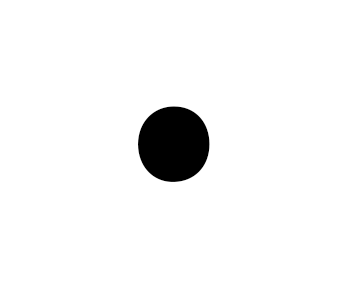
\includegraphics{fig1.png}}
% \caption{Example of a figure caption.}
% \label{fig}
% \end{figure}